% !TEX root = ../thesis.tex
\thispagestyle{plain}
\cleardoublepage
\phantomsection
\addcontentsline{toc}{chapter}{Extended Abstract}
\begin{refsection}

\vspace*{11pt}
\begin{center}
	{\LARGE \textbf{\textsf{Extended Abstract}}}
\end{center}

\bigskip
\begin{center}
	\begin{tabular}{p{3.2cm}p{9.6cm}}
		Titel: & \thema \\
		& \\
		Masterkandidat: & \autor \\
		& \\
		Prüfer: & \firmaA \\ & \firmaB \\[1.1ex] & \prueferA  \\[.5ex]
		&  \prueferB \\
		& \\
		Abgabedatum: & \abgabedatum \\
		& \\
		Schlagworte: & \schlagworte \\
		& \\
	\end{tabular}
\end{center}


\bigskip

\noindent
\textbf{\textsf{Einleitung}}
\vspace*{3pt}

Schwarmverhalten ist eine der grundlegenden Verhaltensmuster in unserer Welt. 
Aufgaben, die für das Individuum unmöglich sind, werden durch die Zusammenarbeit vieler Individuen erst möglich.
Das Verständnis über das Verhalten von Schwärmen kann in vielen technischen Bereichen Fortschritt bedeuten.
Beispielsweise kann das autonome Fahren, bei dem jedes Fahrzeug individuell Entscheidungen trifft, von Schwarmmodellen profitieren.

In dieser Arbeit wird sich mit zwei Schwarmmodellen auseinandergesetzt. Das Ziel ist, mit Hilfe eines Modells Verhaltensmuster eines echten Schwarms abzubilden, indem Parameter für die vorgestellten Modelle geschätzt werden. Dazu wird das Modell auf Realdaten justiert und das Verhalten des Modells dem des echten Schwarms gegenübergestellt.

\vspace*{3pt}
\textbf{\textsf{Methodik}}
\vspace*{3pt}

Um Parameter anhand von Realdaten zu approximieren, werden Trajektorien von Fischschwärmen unterschiedlicher Schwarmgröße verwendet.
Die Daten hierzu sind unter \url{https://idtracker.ai} zu finden.

Als Modell wird ein Boidsmodell \cite{Couzin2002CollectiveMA} und ein eigenes Modell betrachtet. Die Parameter der Modelle werden für das Boidsmodell mit dem Verfahren des Particle Swarm Optimization (PSO) approximiert \cite{PSO_Overview}. Für das eigene Modell wird Reverse Mode Differentiation (RMD) \cite{DBLP:journals/corr/abs-1811-05031} verwendet. Die Verhaltensmuster, welche abgebildet werden sollen, sind die Polarisierung und die Rotation des Schwarms \cite{Tunstrm2013CollectiveSM}

\vspace*{3pt}
\textbf{\textsf{Ergebnisse und Zusammenfassung}}
\vspace*{3pt}

Die Approximation der Parameter hat gezeigt, dass die Schwarmzustände für das eigene Modell abgebildet werden können.

 
\begin{figure}[H]
\centering
\begin{tabular}{cc}
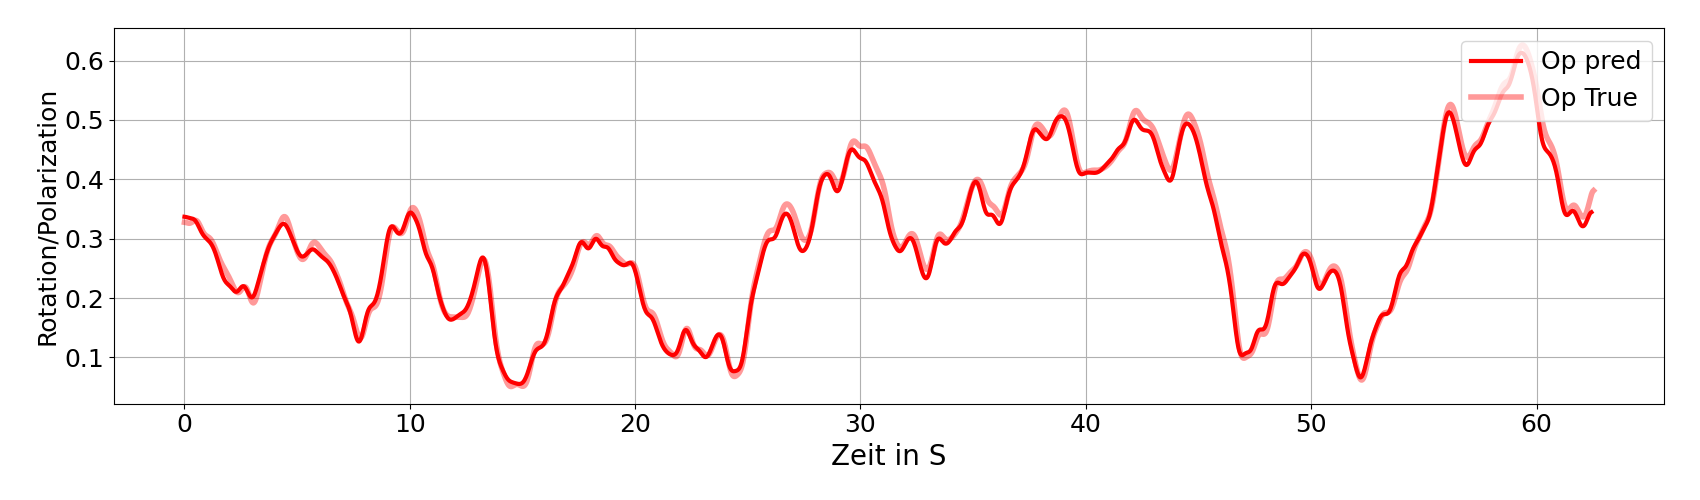
\includegraphics[width=0.5\textwidth]{figures/Experimente/Realdaten/PWD_60Fische_POL.png} &
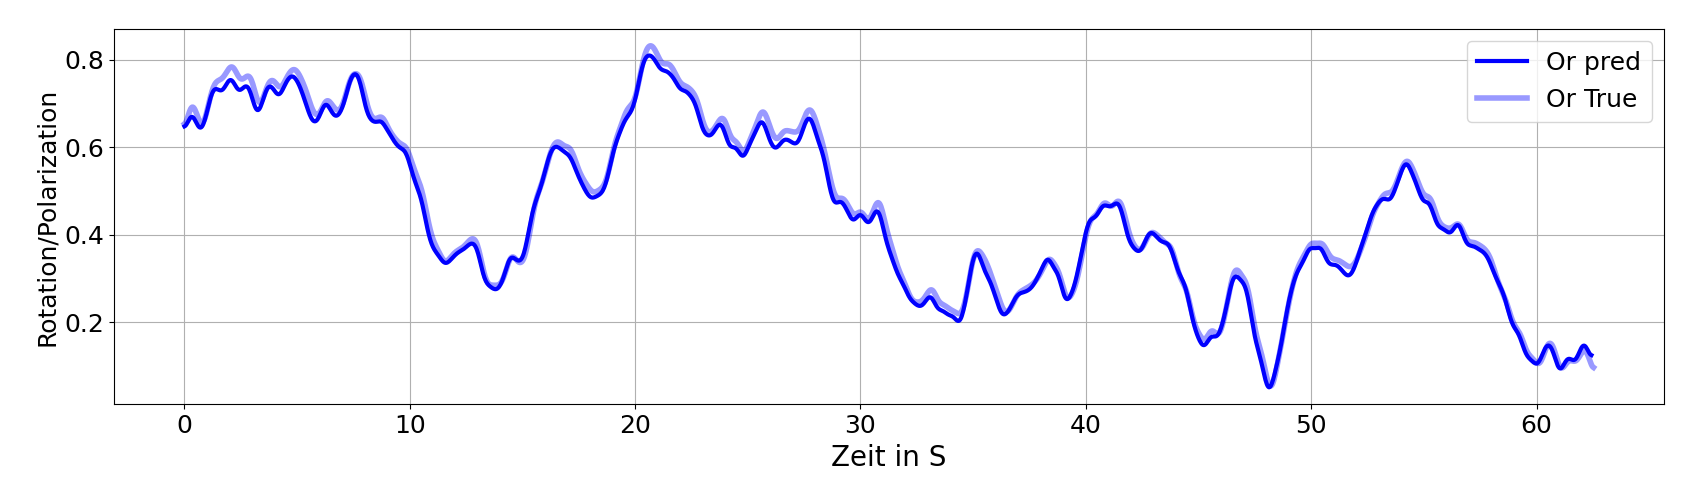
\includegraphics[width=0.5\textwidth]{figures/Experimente/Realdaten/PWD_60Fische_ROT.png} 
\end{tabular}
\caption{Polarisationszustand (links) und Rotationszustand (rechts) der Realdaten mit 60 Fischen und des eigenen Modells\label{fig:60Fisch_rot_EIGEN}}
\end{figure}

Für das Boidsmodell war es nicht möglich die Zustände zu imitieren. 

\begin{figure}[H]
\centering
\begin{tabular}{cc}
\includegraphics[width=0.5\textwidth]{figures/Experimente/Realdaten/Boids_60F_zust_Pol.png} &
\includegraphics[width=0.5\textwidth]{figures/Experimente/Realdaten/Boids_60F_zust_Rot.png} 
\end{tabular}
\caption{Polarisationszustand (links) und Rotationszustand (rechts) der Realdaten mit 60 Fischen und des metrische Boids Modells\label{fig:60Fisch_pol_boids}}
\end{figure}

Auch die Trajektorien zeigen, dass die Approximation für das Boidsmodell in einem unrealistischen Szenario endet.
Das eigene Modell zeigt eine klare Präferenz hinsichtlich der Bewegung und ist ebenfalls vom echten Schwarm zu unterscheiden.

\begin{figure}[H]
\centering
\begin{tabular}{ccc}
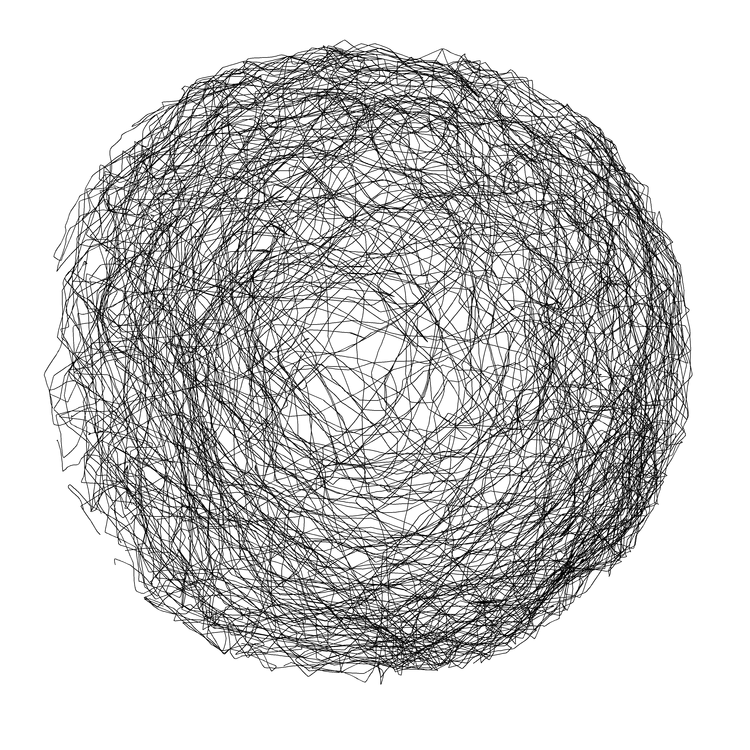
\includegraphics[width=0.33\textwidth]{figures/Experimente/Realdaten/Fisch_60_REAL.png} &
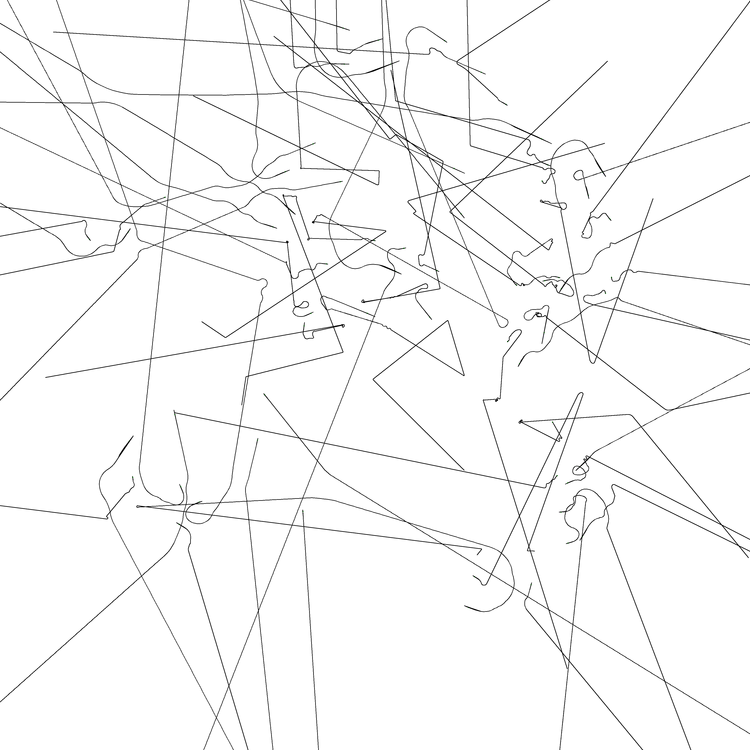
\includegraphics[width=0.33\textwidth]{figures/Experimente/Realdaten/Boids_60_Fisch.png} &
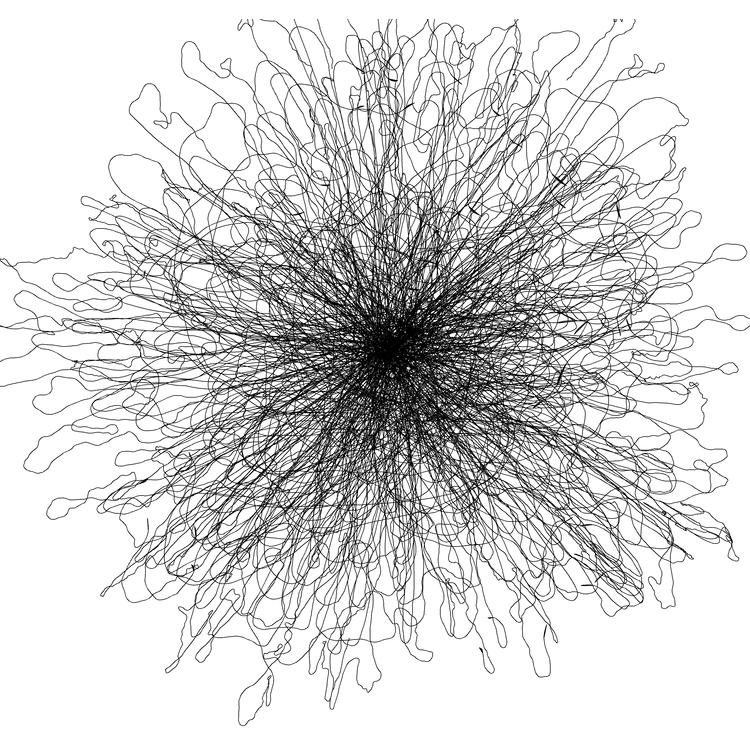
\includegraphics[width=0.33\textwidth]{figures/Experimente/Realdaten/PWD_60_Fisch_sim.png} 
\end{tabular}
\caption{Trajektorien der Realdaten für 60 Fische (links), des metrischen Boids Modells (mitte) und des eigenen Modells (rechts)\label{fig:60FischTraj}}
\end{figure}


\printbibliography[heading=subbibliography]
\end{refsection}


%\section*{Literatur}
